%!TEX root = ../dokumentation.tex

\chapter{Versuchsumgebung}
\label{section:versuchsumgebung}
\todo[inline]{Einführung in Kapitel Versuchsumgebung}
\todo[inline]{Gaze Data Logging hier und Kap 5}

\section{Aufbau}
Um die Verwendung von Eye-Tracking zur Steuerung von Bedienelementen in \ac{VR} untersuchen zu können, finden die Versuche in einem leeren, neutralen Raum statt. Dies hat den Vorteil, dass der Benutzer von der kompletten \ac{VR}-Welt abgeschirmt ist. Der Benutzer kann sich dadurch besser auf den Versuch fokussieren, da dieser nicht durch eventuell neu gewonne Eindrücke aus der \ac{VR}-Welt abgelenkt wird. Um Ablenkungen bezüglich Farbwechsel an den Wänden, dem Boden oder der Decke zu vermeiden, erhalten diese Elemente die selbe Hintergrundfarbe. Zudem wird der Raum gleichmäßig beleuchtet. Für eine bessere Vergleichbarkeit der Versuchsergebnisse muss der Benutzer bei jedem Versuch auf der gleichen Position im Raum stehen. Diese Position wird auf dem Boden durch ein rotes Quadrat markiert (siehe \autoref{fig:game-plan}). Da der Benutzer die Möglichkeit hat, sich innerhalb einer vom \ac{VR}-Headset berechneten Spielfläche zu bewegen, muss sich der Benutzer vor dem Beginn des Versuches auf dem roten Quadrat positionieren. Dieses Quadrat befindet sich mittig zentriert circa eine halbe Einheit vor einer Wand. Das Quadrat hat eine Seitenlänge von einer halben Einheit.

Zur Untersuchung der Eignung von Eye-Tracking bei der Steuerung von Bedienelementen befindet sich auf der gegenüberliegenden Wand die Versuchsfläche (siehe \autoref{fig:game-view}). Der Versuch ist wie ein Spiel aufgebaut. Der Benutzer muss fünf zufällige Zahlen von 1 bis 16 nacheinander auswählen. Auf der Spielfläche befinden sich 16 Bedienelemente, die mit Zahlen von 1 bis 16 beschriftet sind. Oberhalb der Bedienelemente befindet sich ein Textfeld, welches dem Benutzer die auszuwählende Zahl mitteilt. Zudem teilt das Textfeld das Ende des Spieles mit. Um das Spiel zu starten, muss der Benutzer den GO-Button betätigen. Beim Betätigen eines Bedienelementes wird die Hintergrundfarbe des Elements verändert. Dies wird in Abhängigkeit der gesuchten Zahl und des ausgewählten Elements festgelegt. Wenn die gesuchte Zahl und die Beschriftung des ausgewählten Bedienelements übereinstimmen, wird das Element grün gefärbt, ansonsten rot. \\
Für die Untersuchung von Fitts's Law in \ac{VR} sind die Bedienelemente in der Größe verstellbar. Für die Versuche stehen 3 verschiedene Größen zur Verfügung. Während die größte Größe \todo{xx} Einheiten groß ist, ist die mittlere Größe nur halb so groß. Die kleinsten Bedienelemente haben nur noch ein viertel der größten Größe. 

\todo[inline]{Die Aussagen zu der Größe passen nicht !!}

\todo[inline]{Die Zahlen sind nicht zufällig sondern eine zufällige asuwahl von 6 vordefinierten mustern. Die Muster haben alle das gleiche Grundmuster, nur gespiegelt oder versetzt. }
	
\todo[inline]{Im letzten Abschnitt nicht auf die Größe des Kreises sondern auf die Breite/Durchmesser gehen, weil das das interessante für Fitts Law ist.}

\begin{figure}[!htbp]
	\centering
	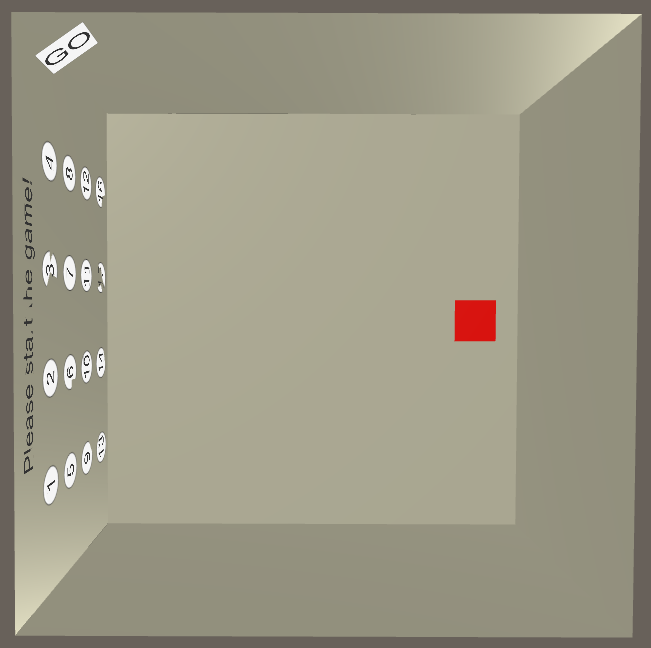
\includegraphics[width=0.65\linewidth]{game-plan}
	\caption[Draufsicht auf den Raum]{Draufsicht auf den Raum}
	\label{fig:game-plan}
\end{figure}

\begin{figure}[!htbp]
\centering
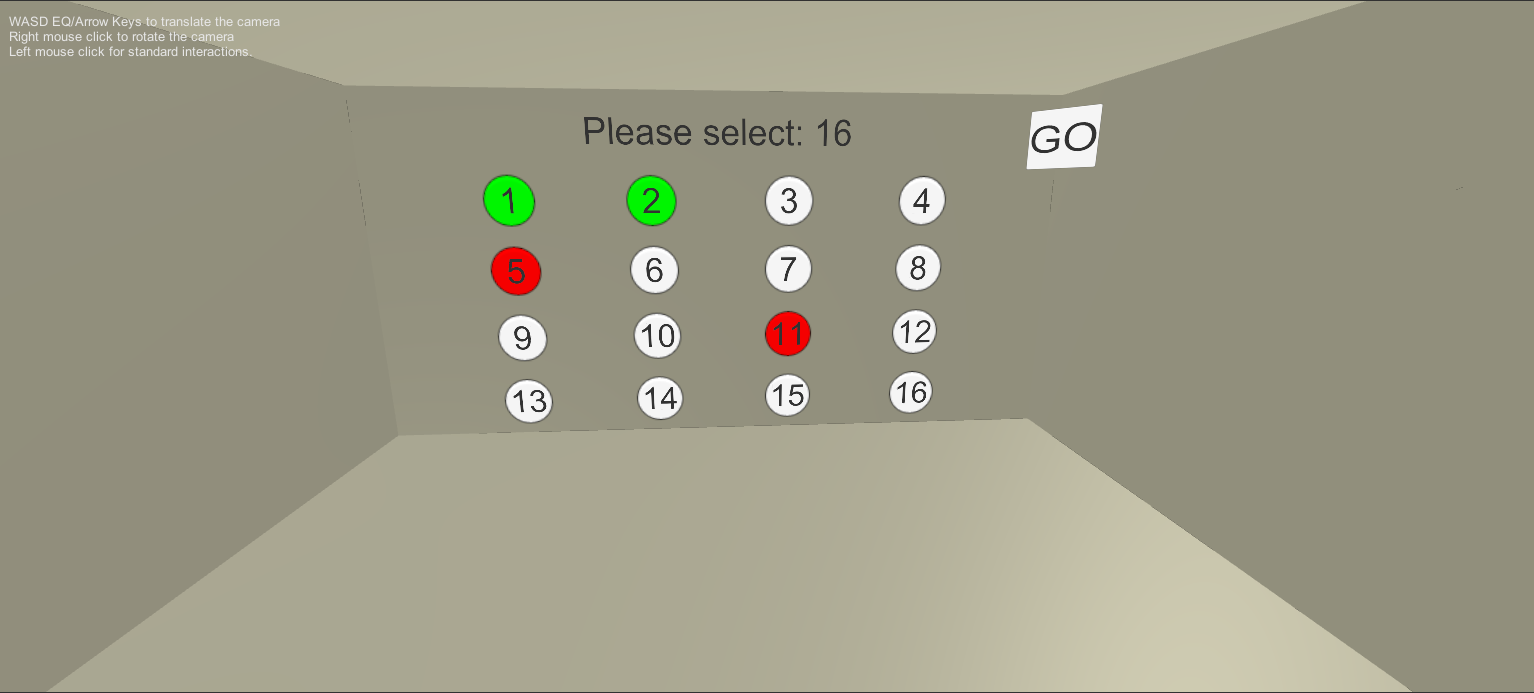
\includegraphics[width=1\linewidth]{game-view}
\caption[Benutzersicht auf den Versuch]{Benutzersicht auf den Versuch}
\label{fig:game-view}
\end{figure}

\section{Szenen}
\todo[inline]{Erklären wieso die Szenen so aufgebaut wurden? Z.B. warum verschiedene Entfernungen? Und wieso das 3D-Level?}
\todo[inline]{Bezug auf Forschungsfrage}
Für die Versuche existieren vier verschiedene Szenen. Jede Szene basiert auf dem zuvor beschriebenen Aufbau. Jeder der Räume ist 2,5 Einheiten hoch und 5 Einheiten breit. Die Idee an den ersten drei Szenen ist zu untersuchen, welchen Einfluss die Entfernung der Bedienelemente auf die Zuverlässigkeit des Eye-Trackings hat. Zudem wird in diesen drei Szenen Fitts' Gesetz in \ac{VR} mit Eye-Tracking untersucht. Die Namen der Szenen orientieren sich daher an Fitts's Law. In der ersten Szene \glqq FittsLaw\grqq (siehe \autoref{fig:game-view}) steht der Benutzer in einer Entfernung von 4,5 Einheiten zur Spielfläche. In der zweiten Szene \glqq FittsLawFar\grqq (siehe \autoref{fig:FittsLawFar}) und der dritten Szene \glqq FittsLawFurther\grqq (siehe \autoref{fig:FittsLawFurther}) vergrößert sich die Entfernung jeweils um 2,5 Einheiten zur vorherigen Szene. In der dritten Szene ist der Benutzer daher 9,5 Einheiten von der Spielfläche entfernt. 

\begin{figure}[!htbp]
	\centering
	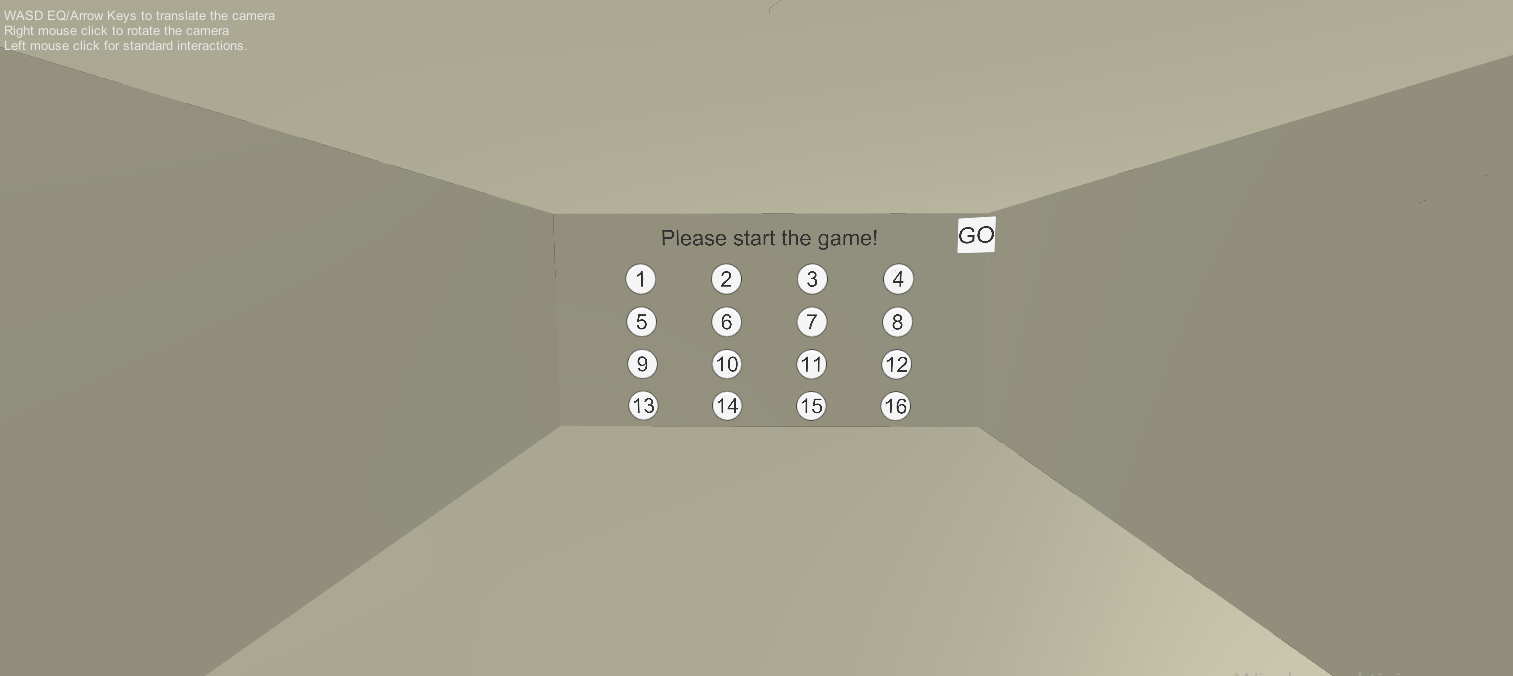
\includegraphics[width=1\linewidth]{FittsLawFar}
	\caption[Szene FittsLawFar]{Szene FittsLawFar}
	\label{fig:FittsLawFar}
\end{figure}

\begin{figure}[!htbp]
	\centering
	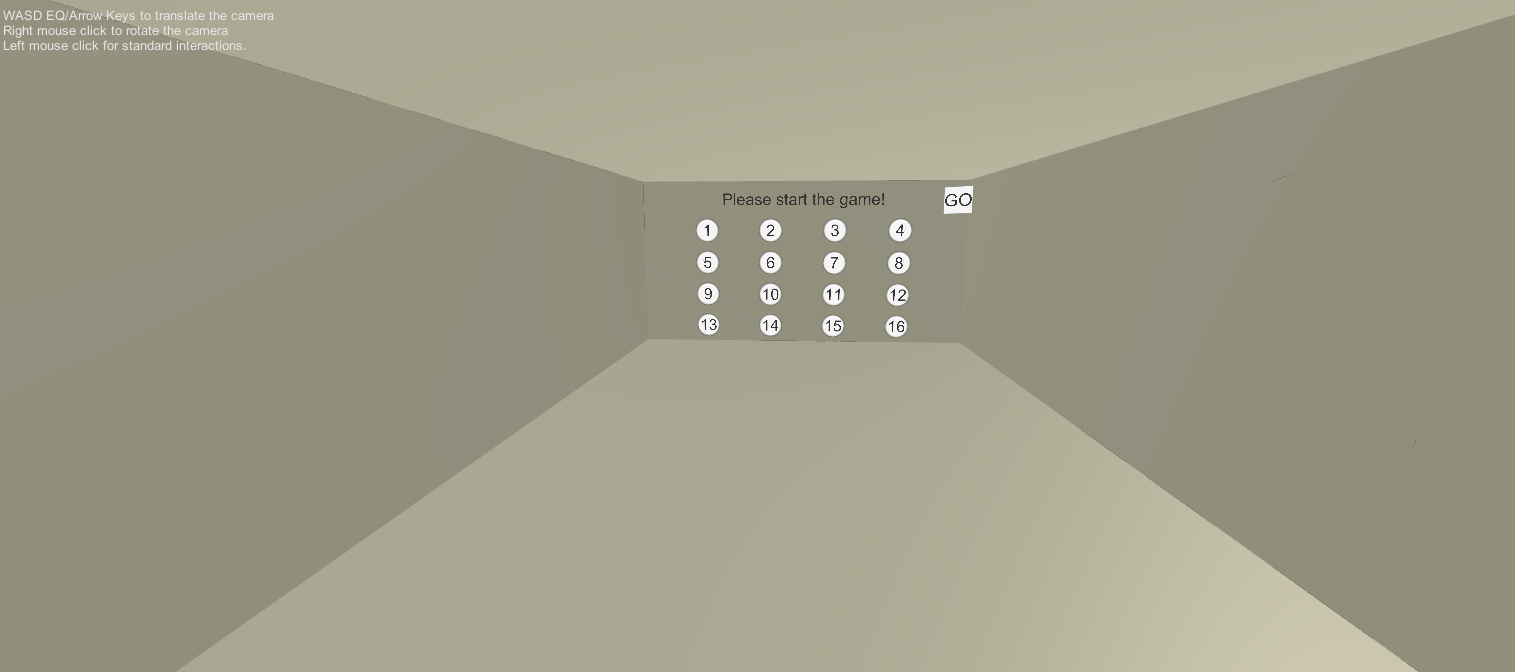
\includegraphics[width=1\linewidth]{FittsLawFurther}
	\caption[Szene FittsLawFurther]{Szene FittsLawFurther}
	\label{fig:FittsLawFurther}
\end{figure}

Bei den ersten drei Szenen ist die Spielfläche zweidimensional. Die Spielfläche befindet sich an der Wand und die Bedienelemente befinden sich auf der gleichen Ebene an der Wand. In der vierten und letzten Szene\glqq 3D-Level\grqq{} (siehe \autoref{fig:3D-Level}) wird untersucht, welche Auswirkungen eine dreidimensionale Spielfläche auf das Eye-Tracking hat. Die Bedienelemente befinden sich nicht mehr auf der gleichen Ebene, sondern schweben im Raum. Die Entfernung zwischen dem Benutzer und den Bedienelementen variiert von 4,5 bis 9,5 Einheiten. Der interessante Aspekt an dieser Szene ist, dass gegebenenfalls ein Bedienelement zum Teil ein anderes Bedienelement verdeckt. Hierbei wird insbesondere die Zuverlässigkeit des Eye-Trackings auf die Probe gestellt. 

\begin{figure}[!htbp]
	\centering
	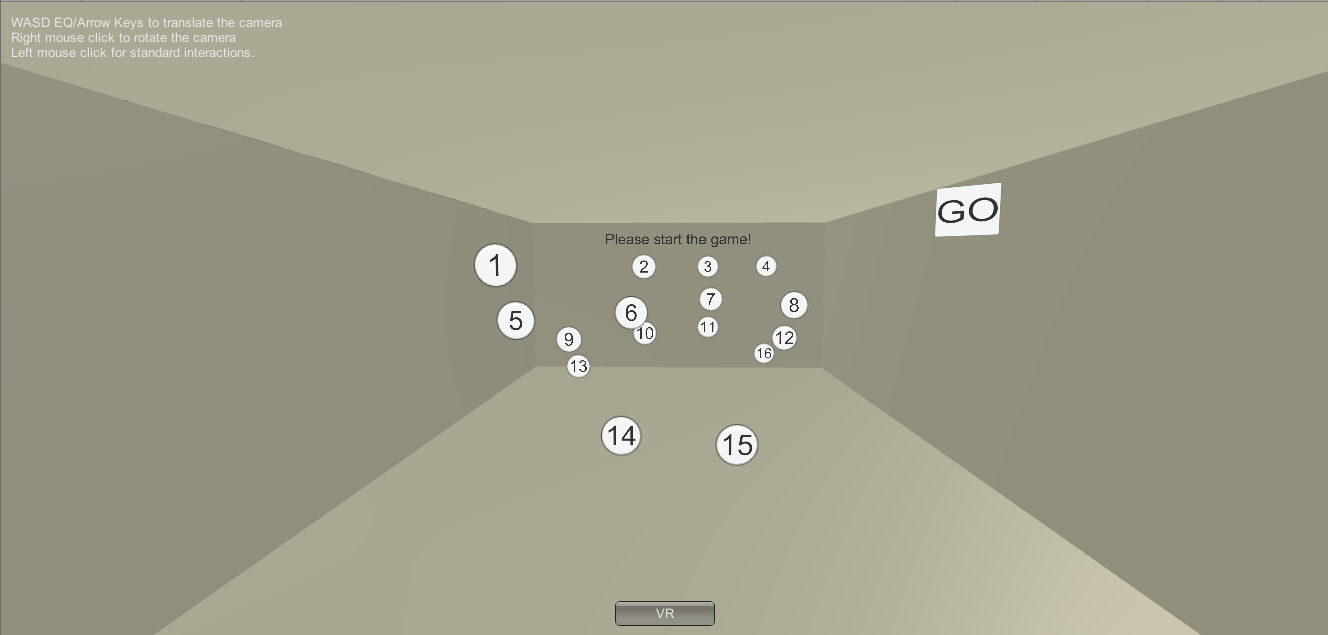
\includegraphics[width=1\linewidth]{3dlevel}
	\caption[Szene 3D-Level]{Szene 3D-Level}
	\label{fig:3D-Level}
\end{figure}

\section{Steuerung}
Um beurteilen zu können, ob sich Eye-Tracking zur Steuerung von Bedienelementen in \ac{VR} eignet, werden verschiedene Steuerungsmöglichkeiten getestet. Die Steuerung innerhalb der \ac{VR}-Umgebung kann mit den Controllern erfolgen und mit dem Eye-Tracking. Die Steuerung lässt sich in Anvisieren und Interagieren unterteilen. Damit beim Anvisieren von Elementen mit dem Controller für den Benutzer klar wird, in welche Richtung der Controller zeigt, wird für das Anvisieren der Controller mit einem Laser versehen. Beim Eye-Tracking wird der Punkt durch eine kleine schwarze Kugel gekennzeichnet, welcher durch den Benutzer anvisiert wird. Das Interagieren mit dem Controller erfolgt durch den Abzug auf der Unterseite des Controllers. Beim Eye-Tracking erfolgt dies durch Blinzeln.\\
Anhand dieser Kenntnisse lassen sich die Steuerungsmöglichkeiten in drei Gruppen aufteilen. Die erste Gruppe ist die Steuerung mit den \ac{VR}-Headset Controllern. Die Controllervariante ist die klassische Steuerungsmöglichkeit. In der Regel benötigt der Benutzer zum Interagieren mit der \ac{VR}-Umgebung mindestens einen Controller. Die zweite Gruppe ist die Steuerung mithilfe des Eye-Trackers. Bei Eye-Tracking wird der Blick zum Anvisieren verwendet und das Blinzeln zum Interagieren mit der \ac{VR}-Umgebung verwendet. Die letzte Möglichkeit ist der Mix aus der klassischen Steuerung sowie der Steuerung mithilfe des Eye-Trackings. Hier übernimmt jeweils eine Steuerungsmöglichkeit das Anvisieren und die andere das Interagieren. Daraus ergeben sich die folgenden vier Versuchskombinationen:

\begin{enumerate}
	\item \textbf{Laser - Trigger}: Diese Versuchskombination verwendet die klassische Steuerelemente in \ac{VR}. Um einschätzen zu können, wie gut Eye-Tracking im Vergleich zu der klassischen Steuerungsvariante funktioniert, wird diese Versuchskombination benötigt. 
	\item \textbf{Blickerfassung - Blink Detection}: Bei dieser Versuchskombination wird der Benutzer nur über Eye-Tracking mit der \ac{VR}-Umgebung interagieren. 
	\item \textbf{Laser - Blink Detection}: Diese Versuchskombination hilft beim Feststellen, wie gut die Interaktion in \ac{VR} mit Blinzeln funktioniert. 
	\item \textbf{Blickerfassung - Trigger}: Bei dieser Versuchskombination liegt der Fokus auf der Blickerfassung. Der Benutzer muss sich nur auf das Anvisieren eines Bedienelementes konzentrieren und mit dem Trigger am Controller die Auswahl betätigen.
\end{enumerate}

\section{Implementierung}
%\begin{wrapfigure}{r}{0.4\textwidth}
%	\vspace{-20pt}
%	\centering
%	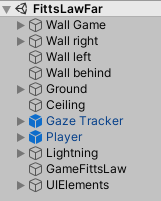
\includegraphics{scenes-structure}
%	\vspace{0pt}
%	\caption[Aufbau der Szenen]{Aufbau der Szenen}
%	\label{fig:scenes-structure}
%	\vspace{-10pt}
%\end{wrapfigure}

\begin{figure}[!htbp]
	\centering
	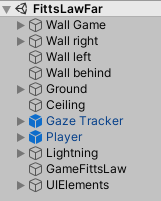
\includegraphics[width=0.4\linewidth]{scenes-structure}
	\caption[Aufbau der Szenen]{Aufbau der Szenen}
	\label{fig:scenes-structure}
\end{figure}

Die \autoref{fig:scenes-structure} zeigt exemplarisch die Objektstruktur der Szenen in Unity. Jede Szene hat 11 Hauptobjekte, welchen teilweise wieder Unterobjekte zugeordnet sind. In der folgenden Aufzählung wird jedes dieser elf Hauptobjekte kurz beschrieben. \todo{macht glaube ich mehr Sinn nur die wichtigsten kurz zu beschreiben}

\begin{description}
	\item \textbf{Wall Game}: Das Objekt ist die Wand gegenüber des Spielers. Diese Wand ist die Spielfläche, weshalb die Buttons der Wand als Unterobjekte zugeordnet sind. 
	\item \textbf{Wall right}: Das Objekt ist die Wand auf der rechten Seite des Spielers, wenn dieser sein Blick zur Spielfläche wendet. Dieser Wand ist der GO-Button zugeordnet.
	\item \textbf{Wall left}: Dieses Objekt ist die Wand auf der linken Seite des Spielers.
	\item \textbf{Wall behind}: Dieses Objekt stellt die Wand hinter dem Spieler dar.
	\item \textbf{Ground}: Das Objekt ist der Boden. Als Unterobjekt ist das rote Quadrat enthalten, auf dem sich der Spieler vor den Versuchen zu positionieren hat.
	\item \textbf{Ceiling}: Das Objekt ist die Decke.
	\item \textbf{Gaze Tracker}: Der GazeTracker enthält die relevanten Informationen für das Eye-Tracking. In diesem Objekt wird zudem die Kommunikation zum Eyetracker von Pupil Labs hergestellt.
	\item \textbf{Player}: Das Spielerobjekt enthält die relevanten Informationen, welche für den Spieler wichtig sind. Dieses Objekt nutzt zudem die Schnittstelle zu SteamVR. 
	\item \textbf{Lightning}: Das Objekt beinhaltet die Objekte für die Beleuchtung für den Raum. Für eine angenehme gleichmäßige Beleuchtung im Raum werden zwei Point Lights verwendet. Die Lichter sind in der Mitte des Raumes jeweils einmal an der Decke und an dem Boden angebracht. 
	\item \textbf{GameFittsLaw}: Dieses Objekt beinhaltet die Spiellogik. Es ist daher nicht sichtbar in der \ac{VR}-Umgebung.
	\item \textbf{UIElements}: Diesem Objekt sind die graphischen Elemente für die verschiedenen Einstellungen für die Versuche zugeordnet.
\end{description}

In \autoref{fig:ClassDiagram} ist ein Überblick der für dieses Projekt generierten Klassen und der Hierarchie dargestellt. Gut zu sehen ist, dass durch Vererbung der Großteil der Klassen die Unity eigene Klasse MonoBehaviour ist. Nachfolgend werden die wichtigsten Objekte beziehungsweise Strukturen erläutert. 

\subsection{Player}
\todo{Player}

\subsection{Gaze Tracker}
\todo{Gaze Tracker}
Gaze Visualizer??? --> Wird in Subkapitel Measurement benötigt.
BaseMono???

\subsection{UIElements}
Damit für jede Versuchskombination nicht eine eigene Umgebung erstellt werden muss, erhält jede Umgebung eine Einstellungsmöglichkeit für die verschiedenen Versuchskombinationen. In \autoref{fig:switch-different-options} ist die Einstellungsoberfläche für die Versuchskombinationen dargestellt. Für die Versuche können sowohl die Steuerungskombinationen als auch die Durchmesser der Buttons verändert werden. Zur Fixierung eines Objektes kann entweder der Laser oder das Eye-Tracking verwendet werden. Die Bestätigung kann entweder über den Trigger am Controller oder Blink Detection erfolgen. Mit dem unteren Slider lässt sich der Durchmesser der Buttons verändern. 

\begin{figure}[!htbp]
	\centering
	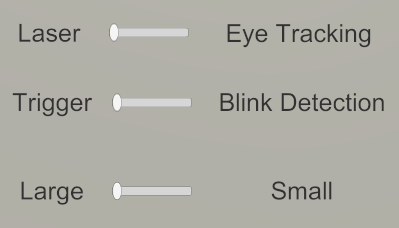
\includegraphics[width=1\linewidth]{switch-different-options}
	\caption[Einstellungsoberfläche für die Versuchsoptionen]{Einstellungsoberfläche für die Versuchsoptionen; Oben: Anvisieren; Mitte: Bestätigen; Unten: Größe der Buttons}
	\label{fig:switch-different-options}
\end{figure}

Sowohl für die Steuerungsmöglichkeit als auch für die Skalierung der Buttondurchmesser werden Enumerationen verwendet, die die verschiedenen Status darstellen. Zudem wurde zu jeder Enumeration zusätzlich eine Property-Klasse angelegt. Das Ziel mit der Property-Klasse ist es, die aktuell gültige Steuerungskombination sowie die Skalierung der Buttons global zu sichern. Außerdem soll jede Klasse, die Kenntnisse über die Daten hat, bei Änderungen des Wertes über ein PropertyChanged-Event informiert werden. Die Klassen haben somit bei Interesse an den Werten die Möglichkeit das Event zu abonnieren. \\
Wie in \autoref{fig:ClassDiagrammProperties} zu sehen gibt es die Enumerationen ControlState und Scaling. ControlState beinhaltet die Enumerationen LaserTrigger, EyeTrigger, LaserBlinking und BlinkingEye. Scaling beinhaltet die Enumerationen Large, Medium und Small. Zu jeder Enumeration existiert zudem die passende Property-Klasse. Während ControlStateProperty nur den aktuellen Wert von ControlState speichert, wird in ScalingProperty neben dem aktuellen Scaling Wert zusätzlich Faktoren für die Höhe, Breite und Tiefe bei den unterschiedlichen Scalings gespeichert. Während bei Large der Faktor eins beträgt, ist der Faktor bei Small nur noch halb so groß. \todo{Genaue Erklärung wieso 1/sqrt(2)}

\begin{figure}[!htbp]
	\centering
	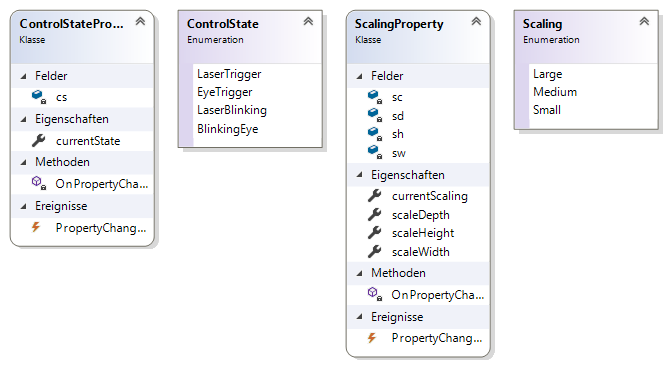
\includegraphics[width=1\linewidth]{ClassDiagramProperties}
	\caption[Klassendiagramm der ScalingProperty \& ControlStateProperty]{Klassendiagramm der ScalingProperty \& ControlStateProperty}
	\label{fig:ClassDiagrammProperties}
\end{figure}

Ein Slider feuert ein On Value Changed Event, sobald sich der Wert des Sliders ändert. Diese Events werden in der Klasse BasePlayer abgefangen. Diese Events werden in der Klasse BasePlayer abgefangen und verarbeitet. In \autoref{LaserEyeTracking} ist die Methode LaserEyeTrackingSliderChanged, welche Änderungen des ersten Sliders zwischen Laser und EyeTracking abfängt. Obwohl in der Methode der neue Wert nicht mitgeliefert werden kann, kann der neue Wert gesetzt werden. Hier wird sich der Eigenschaft einer Enumeration zunutze gemacht, in der der Datentyp des Konstantenwerts der Enumerationsmember ein Integer ist \cite{BillWagner.2020}. Mithilfe von geschickter XOR Arithmetik kann der Status in ControlState gesetzt werden. Da vier Werte vorhanden sind reichen zwei Bits aus um die Kombinationen zu erstellen. Für das Fokussieren auf ein Objekt wird die niederwertigste Bit-Stelle verwendet. Wenn das Bit 0 ist, wird der Laser zum fokussieren verwendet, bei einer 1 das Eye-Tracking. Bei der höherwertigen Bit-Stelle wird das Bestätigen der Auswahl gesetzt. Eine 0 ist das Verwenden des Abzuges, eine 1 des Blinzelns. Beim Slider für das Scaling werden dem Slider die Werte 0, 1 und 2 zugewiesen. Durch Casten \todo{Mir fällt jetzt kein deutsches Wort zu ein} des Datentyps von Integer zur Enumeration erhält man das aktuelle Scaling.

\begin{lstlisting}[caption=Method LaserEyeTrackingSliderChanged,label=LaserEyeTracking]
public void LaserEyeTrackingSliderChanged()
{
    int state = (int)ControlStateProperty.currentState;
    state = state ^ 0b01;
    this.setControlState((ControlState)state);
}
\end{lstlisting}

\subsection{Buttons}
\blindtext
\begin{figure}[!htbp]
	\centering
	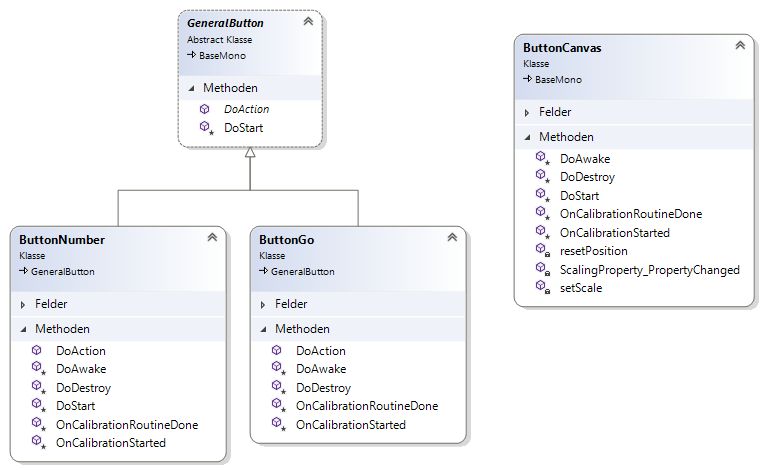
\includegraphics[width=1\linewidth]{ClassDiagramButton}
	\caption[Klassendiagramm Button]{Klassendiagramm Button}
	\label{fig:ClassDiagramButton}
\end{figure}

\subsection{Game}
%\begin{figure}[!htbp]
%	\centering
%	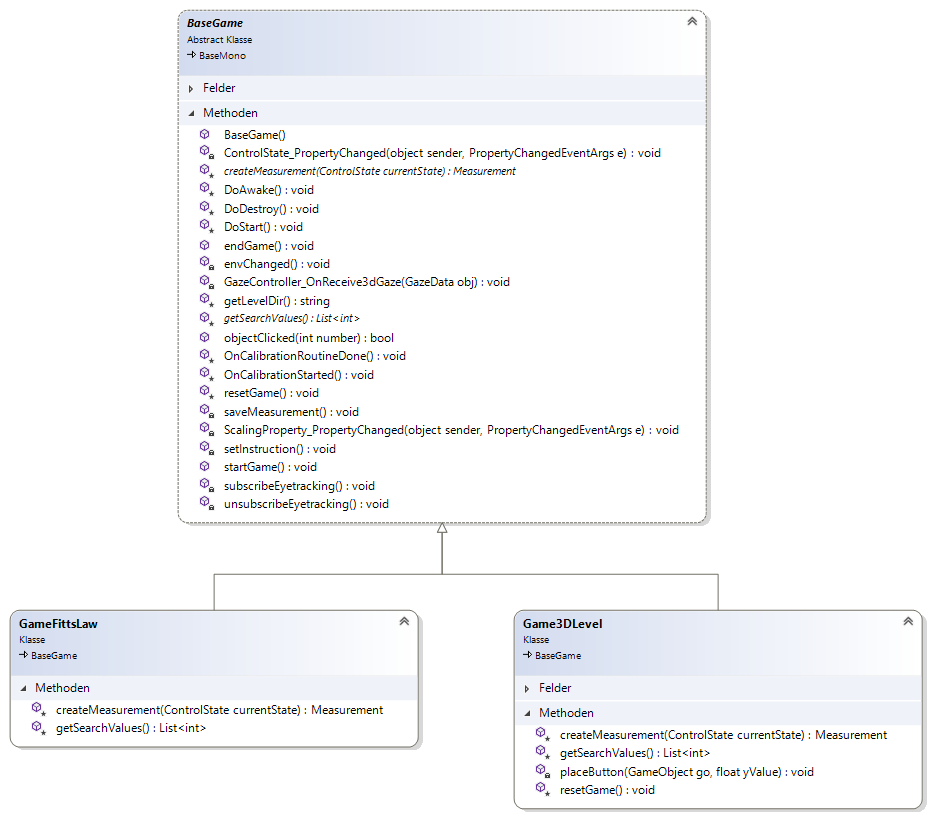
\includegraphics[width=1\linewidth]{ClassDiagramGame}
%	\caption[Klassendiagramm Game]{Klassendiagramm Game}
%	\label{fig:ClassDiagramGame}
%\end{figure}

Wände haben -1; Buttons die entsprechende Zahl

3DLevel Buttons verschieben

\subsection{Measurement}
Um einen Vergleich zwischen den Steuerungsmöglichkeiten ziehen zu können, werden die Versuche aufgezeichnet. In \autoref{fig:ClassDiagramMeasurement} ist der Ausschnitt der Klassen für die Measurements zu sehen. Zu jeder Messung wird das aktuelle Level, die verwendete Steuerungskombination sowie die Skalierung der Buttons eines Versuchs gespeichert. Am Anfang sowie am Ende der Messung wird jeweils der aktuelle Zeitpunkt gespeichert. Hierdurch ist es möglich die Dauer des Versuchs zu berechnen. Die Zeit wird in der Messung als Zeitstempel in Millisekunden gesichert. In dem Feld action werden die durch den Benutzer getätigten Bestätigungen durch den Abzug beziehungsweise mithilfe von Blinzeln erfasst. Hierbei wird der Zeitstempel, die Nummer des Buttons sowie ob es der gesuchte Button war gespeichert. \todo{Mal schauen wo ich das mit der -1 bei ner Wand erkläre.} Die Daten werden als String mit Komma getrennt in einer Liste gespeichert. Für Fitts Law ist bei der Verwendung von Eye-Tracking der Verlauf des Blickes interessant. Aus diesem Grund wird der Blickverlauf mit gemessen. Die Blickdaten werden ebenfalls in einer Liste bestehend aus Strings gespeichert. Da die Blickdaten als 3D-Vektor vorliegen, werden die Koordinaten des durch den Blick fixierten Punktes mit Komma getrennt aufgezeichnet. Alle 100 ms werden die Blickdaten erfasst und gesichert. Als Datengrundlage für die Blickverfolgung dient der Gaze Visualizer vom Gaze Tracker. Für das 3D-Level werden zusätzlich die Positionen und der Buttons aufgezeichnet. Dies wird benötigt, da sich die Position der Buttons im Raum von Versuch zu Versuch unterscheiden. Für die Zuordnung, welcher Button auf welcher Position steht, werden zusätzlich die Nummern der Buttons mit gespeichert.

\begin{figure}[!htbp]
	\centering
	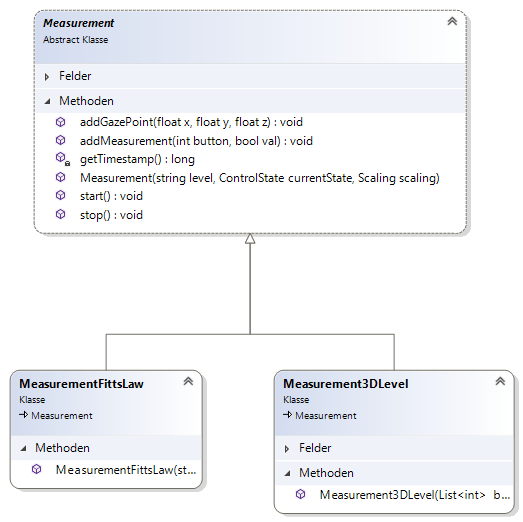
\includegraphics[width=0.75\linewidth]{ClassDiagramMeasurement}
	\caption[Klassendiagramm Measurements]{Klassendiagramm Measurements}
	\label{fig:ClassDiagramMeasurement}
\end{figure}

Jede Messung wird am Ende eines Versuchs in einer JSON-Datei abgespeichert. Die Basisklasse Measurement ist mit dem Attribut Serializable gekennzeichnet. Dies ermöglicht das Serialisieren des kompletten Measurement-Objekts. Damit alle Messdaten mit dem Objekt serialisiert werden müssen die Felder als öffentlich gekennzeichnet sein. Das Serialisieren in ein JSON-String wird mithilfe von Unity bereitgestellten Klasse JsonUtility durchgeführt. Für eine Gliederung der Messungen werden die Messungen in unterschiedlichen Ordnern nach Level und verwendeter Skalierung getrennt gespeichert. Der Dateiname ist zudem der Zeitstempel zum Zeitpunkt des Speichervorganges der Messung.